\chapter{Simple Line Plots\label{Ch26}}

\begin{tcolorbox}
    In Matplotlib, the figure (an instance of the class plt.Figure) can be thought of as a
    single container that contains all the objects representing axes, graphics, text, and
    labels. The axes (an instance of the class plt.Axes) is what we see above: a bounding
    box with ticks, grids, and labels, which will eventually contain the plot elements that
    make up our visualization. Throughout this part of the book, I'll commonly use the
    variable name fig to refer to a figure instance and ax to refer to an axes instance or
    group of axes instances.
\end{tcolorbox}

Once we have created an axes, we can use the ax.plot method to plot some data.

Alternatively, we can use the PyLab interface and let the figure and axes be created for
us in the background.
\section{Adjusting the Plot: Line Colors and Styles}
The first adjustment you might wish to make to a plot is to control the line colors and
styles. The plt.plot function takes additional arguments that can be used to specify
these. To adjust the color, you can use the \verb|color|\marginpar[color]{color} keyword, which accepts a string
argument representing virtually any imaginable color. The color can be specified in a
variety of ways.

\begin{pyc}
    plt.plot(x, np.sin(x - 0), color='blue')        # specify color by name
    plt.plot(x, np.sin(x - 1), color='g')           # short color code (rgbcmyk)
    plt.plot(x, np.sin(x - 2), color='.75')         # grayscale between 0 and 1
    plt.plot(x, np.sin(x - 3), color='#FFDD44')     # hex code (RRGGBB, 00 to FF)
    plt.plot(x, np.sin(x - 4), color=(1.0, .2, .3)) # RGB tuple, values 0 to 1
    plt.plot(x, np.sin(x - 5), color='chartreuse')  # HTML color names supported
\end{pyc}

If no color is specified, Matplotlib will automatically cycle through a set of default
colors for multiple lines.

Similarly, the line style can be adjusted using the \verb|linestyle|\marginpar[linestyle]{linestyle} keyword.

\begin{pyc}
    plt.plot(x, x + 0, linestyle='solid')
    plt.plot(x, x + 1, linestyle='dashed')
    plt.plot(x, x + 2, linestyle='dashdot')
    plt.plot(x, x + 3, linestyle='dotted')

    # For short, you can use the following codes:
    plt.plot(x, x + 4, linestyle='-')  # solid
    plt.plot(x, x + 5, linestyle='--') # dashed
    plt.plot(x, x + 6, linestyle='-.') # dashdot
    plt.plot(x, x + 7, linestyle=':'); # dotted
\end{pyc}

Though it may be less clear to someone reading your code, you can save some key-strokes by combining these linestyle and color codes into a single non-keyword
argument to the plt.plot function:

\begin{pyc}
    plt.plot(x, x + 0, '-g')  # solid green
    plt.plot(x, x + 1, '--c') # dashed cyan
    plt.plot(x, x + 2, '-.k') # dashdot black
    plt.plot(x, x + 3, ':r')  # dotted red
\end{pyc}

These single-character color codes reflect the standard abbreviations in the RGB
(Red/Green/Blue) and CMYK (Cyan/Magenta/Yellow/blacK) color systems, commonly used for digital color graphics.

\section{Adjusting the Plot: Axes Limits}
Matplotlib does a decent job of choosing default axes limits for your plot, but sometimes it's nice to have finer control. The most basic way to adjust the limits is to use
the plt.xlim\marginpar[plt.xlim]{plt.xlim} and plt.ylim\marginpar[plt.ylim]{plt.ylim} functions.

If for some reason you'd like either axis to be displayed in reverse, you can simply
reverse the order of the arguments.

A useful related method is \verb|plt.axis|\marginpar[plt.axis]{plt.axis} (note here the potential confusion between axes
with an e, and axis with an i), which allows more qualitative specifications of axis limits.(自动收紧坐标轴,不留空白区域)

Or you can specify that you want an equal axis ratio, such that one unit in x is visually
equivalent to one unit in y. Other axis options include 'on', 'off', 'square', 'image', and more. For more
information on these, refer to the plt.axis docstring.

\section{Labeling Plots}
We'll briefly look at the labeling of plots: titles, axis
labels, and simple legends. Titles and axis labels are the simplest such labels—there
are methods that can be used to quickly set them. The position, size, and style of these labels can be adjusted using optional arguments
to the functions, described in the docstrings.

When multiple lines are being shown within a single axes, it can be useful to create a
plot legend that labels each line type. Again, Matplotlib has a built-in way of quickly
creating such a legend; it is done via the \verb|plt.legend| method.
Though there are several valid ways of using this, I find it easiest to specify the label
of each line using the label keyword of the plot function.

\section{Matplotlib Gotchas}
While most plt functions translate directly to ax methods (plt.plot $\rightarrow$ ax.plot,
plt.legend $\rightarrow$ ax.legend, etc.), this is not the case for all commands. In particular,
functions to set limits, labels, and titles are slightly modified. For transitioning
between MATLAB-style functions and object-oriented methods, make the following
changes:
\begin{itemize}
    \item \verb|plt.xlabel| $\rightarrow$ \verb|ax.set_xlabel|
    \item \verb|plt.ylabel| $\rightarrow$ \verb|ax.set_ylabel|
    \item \verb|plt.xlim| $\rightarrow$ \verb|ax.set_xlim|
    \item \verb|plt.ylim| $\rightarrow$ \verb|ax.set_ylim|
    \item \verb|plt.title| $\rightarrow$ \verb|ax.set_title|
\end{itemize}

In the object-oriented interface to plotting, rather than calling these functions individually, it is often more convenient to use the \verb|ax.set| method to set all these properties at once.

\begin{figure}[H]
    \centering
    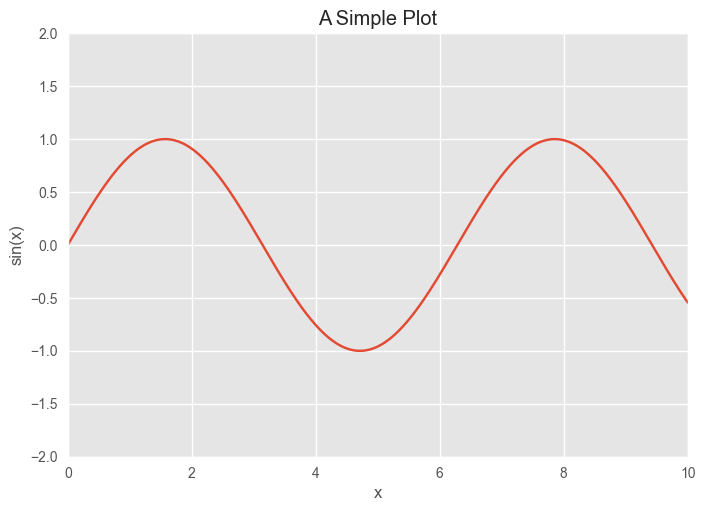
\includegraphics{../Figures/fig26-14.png}
    \caption{Example of using \texttt{ax.set} to set multiple properties at once}
    \label{fig26-14}
\end{figure}

\begin{pyc}
    ax = plt.axes()
    ax.plot(x, np.sin(x))
    ax.set(xlim=(0, 10), ylim=(-2, 2), xlabel='x', ylabel='sin(x)', title='A Simple Plot')
\end{pyc}